%\chapter{Desenvolvimento}
\label{desenvolvimento}
\section{Inserção}
Como dito anteriormente, a implementação desta arvore segue a logica de que seriam inseridos arquivos de 1kB e de 256B, considerando também que o tamanho de um setor na unidade de armazenamento contém 512 Bytes, e uma página contém 4 kB.
Isso resultou em 2 modelos de arvores para cada tipo, ou seja 2 arvores B instanciadas para receber sucessivamente arquivos de 1kB em uma e arquivos de 256B na outra. O mesmo caso ocorre nas arvores B*.

Logo as características resultantes destas arvores foram:\\
\begin{center}
Arvore B - 1: m = 4;\\
Arvore B - 2: m = 8;\\
Arvore B* - 1: m = 4;\\
Arvore B* - 2: m = 8.
\end{center}

Os arquivos inseridos são representados por objetos do tipo MeuItem desenvolvido também pelo professor e pesquisador da UFMG, Nivio Ziviani. este objeto armazena um inteiro que foi gerado de forma pseudoaleatória utilizando de um algoritmo para esse fim.  


\subsection{Arvore B - Arquivos 1kB}

\begin{figure}[ht]
    \centering
    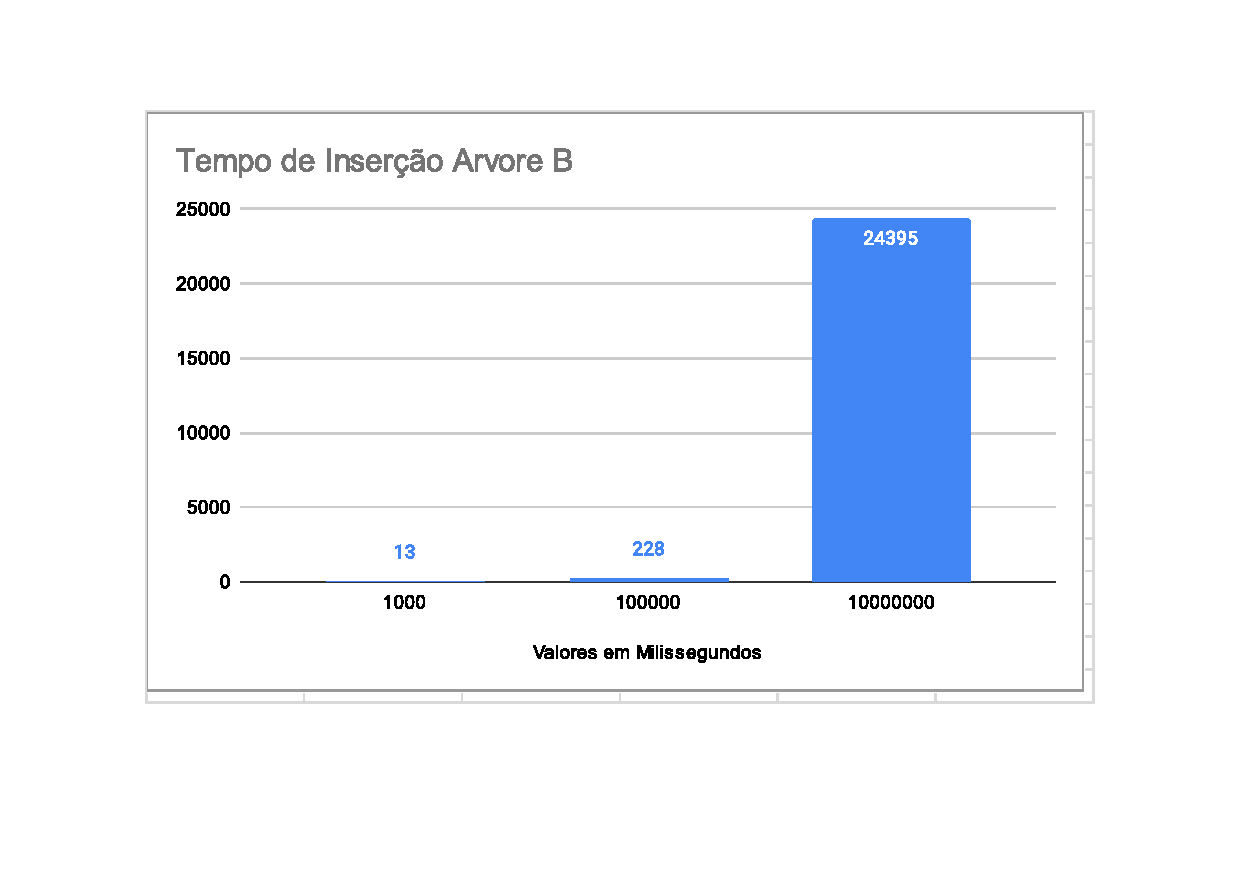
\includegraphics[scale=0.6]{Trabalho AED/fig/Planilha sem título - Página2.pdf}
    \label{fig:my_label}
\end{figure}
\begin{center}
        \begin{tabular}{| l | r |}
            \hline
            Quantidade de arquivos & Tempo em Milissegundos\\
            \hline
            10\textsuperscript{3} & 13\\
            10\textsuperscript{5} & 228\\
            10\textsuperscript{7} & 24395\\
            \hline
        \end{tabular}
    \end{center}
\subsection{Arvore B - Arquivos 256B}

\begin{figure}[ht]
    \centering
    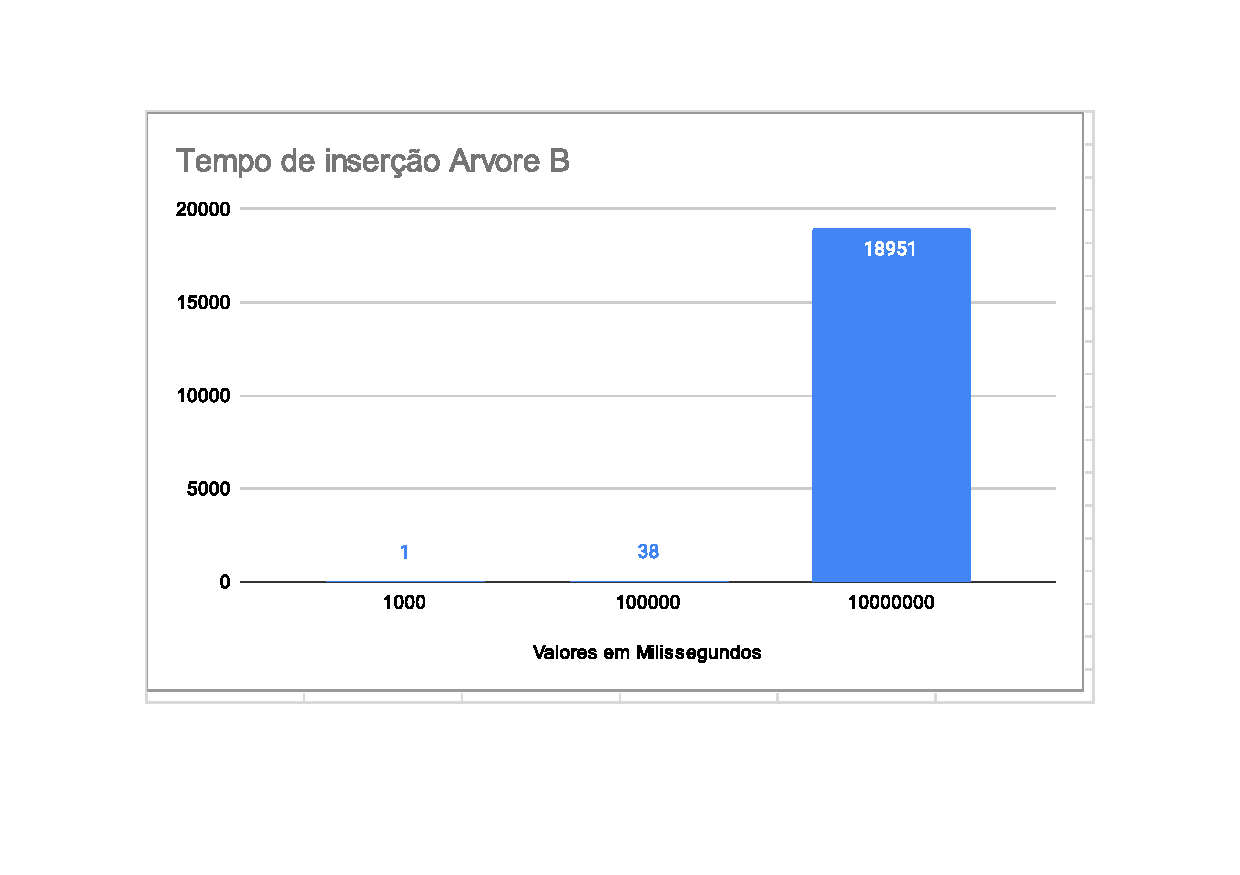
\includegraphics[scale=0.6]{Trabalho AED/fig/Planilha sem título - Página4 (1).pdf}
    \label{fig:my_label}
\end{figure}
\begin{center}
        \begin{tabular}{| l | r |}
            \hline
            Quantidade de arquivos & Tempo em Milissegundos\\
            \hline
            10\textsuperscript{3} & 1\\
            10\textsuperscript{5} & 38\\
            10\textsuperscript{7} &  18951\\
            \hline
        \end{tabular}
    \end{center}


\subsection{Arvore B* - Arquivos 1kB}

\subsection{Arvore B* - Arquivos 256B}


\section{Remoção}

Após o processo de inserção daqueles objetos que representam os arquivos a serem inseridos na arvore, são executados testes de tempo de remoção de 5\% dos mesmos. Gerando os seguintes resultados a seguir:

\subsection{Arvore B - Arquivos 1kB}

\begin{figure}[ht]
    \centering
    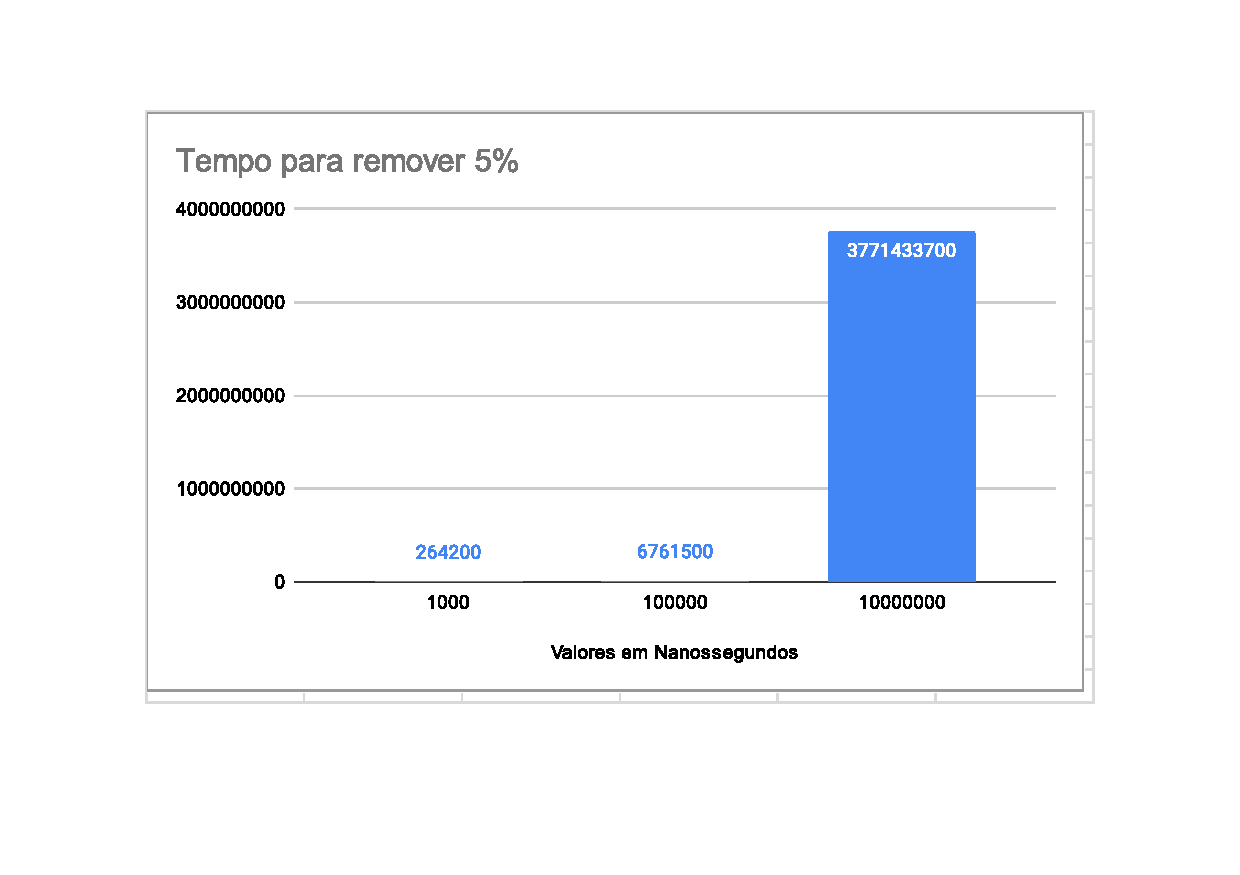
\includegraphics[scale=0.6]{Trabalho AED/fig/Planilha sem título - Página6.pdf}
    \label{fig:my_label}
\end{figure}
 \begin{center}
        \begin{tabular}{| l | r |}
            \hline
            Quantidade de arquivos & Tempo em Nanossegundos\\
            \hline
            10\textsuperscript{3} & 264200\\
            10\textsuperscript{5} &  6761500\\
            10\textsuperscript{7} &  3771433700 \\
            \hline
        \end{tabular}
    \end{center}
\subsection{Arvore B - Arquivos 256B}

\begin{figure}[ht]
    \centering
    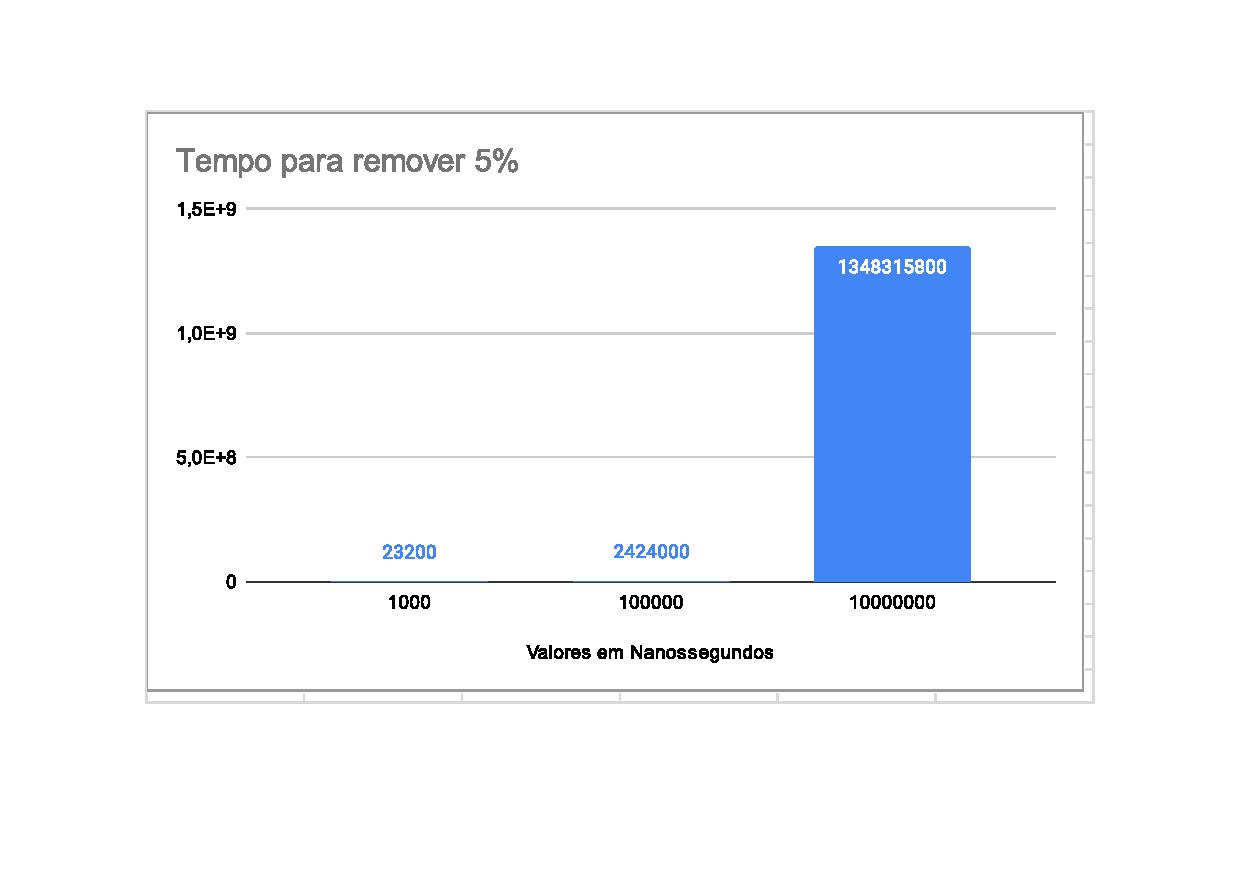
\includegraphics[scale=0.6]{Trabalho AED/fig/Planilha sem título - Página8.pdf}
    \label{fig:my_label}
\end{figure}
 \begin{center}
        \begin{tabular}{| l | r |}
            \hline
            Quantidade de arquivos & Tempo em Nanossegundos\\
            \hline
            10\textsuperscript{3} & 23200 \\
            10\textsuperscript{5} & 2424000\\
            10\textsuperscript{7} &  1348315800 \\
            \hline
        \end{tabular}
    \end{center}
\subsection{Arvore B* - Arquivos 1kB}

\subsection{Arvore B* - Arquivos 256B}